\documentclass[xcolor=pdflatex,dvipsnames,table]{beamer}
\usepackage{epsfig,graphicx}
\usepackage{palatino}
\usepackage{fancybox}
\usepackage{relsize}
\usepackage[procnames]{listings}
\usepackage{hyperref}
\usepackage{qtree} % needed?
\usepackage{booktabs}
\usepackage{dirtree}
\usepackage[normalem]{ulem}


% fatter TT font
\renewcommand*\ttdefault{txtt}
% another TT, suggested by Alex
% \usepackage{inconsolata}
% \usepackage[T1]{fontenc} % needed as well?


\newcommand{\scale}{0.7}

\newcommand{\todo}[1]{{\emph{TODO: #1}}}
\newcommand{\martin}[1]{{\color{blue} Martin: #1}}
\newcommand{\abcdef}[1]{{\color{red} Author2: #1}}

% uncomment following for final submission
%\renewcommand{\todo}[1]{}
%\renewcommand{\martin}[1]{}
%\renewcommand{\author2}[1]{}

\newcommand{\code}[1]{{\texttt{#1}}}

\hypersetup{
  linkcolor  = black,
%  citecolor  = blue,
  urlcolor   = blue,
  colorlinks = true,
}

\beamertemplatenavigationsymbolsempty
\setbeamertemplate{footline}[frame number]





\newif\ifbook
% shared in slides and book

\lstdefinelanguage{chisel}{
%  morekeywords={abstract,case,catch,class,def,%
%    do,else,extends,false,final,finally,%
%    for,if,implicit,import,match,mixin,%
%    new,null,object,override,package,%
%    private,protected,requires,return,sealed,%
%    super,this,throw,trait,true,try,%
%    type,val,var,while,with,yield},
%  otherkeywords={=>,<-,<\%,<:,>:,\#,@},
  sensitive=true,
  morecomment=[l]{//},
  morecomment=[n]{/*}{*/},
  morestring=[b]",
  morestring=[b]',
  morestring=[b]"""
}

\usepackage{color}
\definecolor{dkgreen}{rgb}{0,0.6,0}
\definecolor{gray}{rgb}{0.5,0.5,0.5}
\definecolor{mauve}{rgb}{0.58,0,0.82}

% Default settings for code listings
%\ifbook
\lstset{%frame=lines,
  language=chisel,
  aboveskip=3mm,
  belowskip=3mm,
  showstringspaces=false,
  columns=fixed, % basewidth=\mybasewidth,
  basicstyle={\small\ttfamily},
  numbers=none,
  numberstyle=\footnotesize,
  % identifierstyle=\color{red},
  breaklines=true,
  breakatwhitespace=true,
  procnamekeys={def, val, var, class, trait, object, extends},
  % procnamestyle=\ttfamily,
  tabsize=2,
  float
}
%\else
%\lstset{%frame=lines,
%  language=chisel,
%  aboveskip=3mm,
%  belowskip=3mm,
%  showstringspaces=false,
%  columns=fixed, % basewidth=\mybasewidth,
%  basicstyle={\small\ttfamily},
%  numbers=none,
%  numberstyle=\footnotesize\color{gray},
%  % identifierstyle=\color{red},
%  keywordstyle=\color{blue},
%  commentstyle=\color{dkgreen},
%  stringstyle=\color{mauve},
%  breaklines=true,
%  breakatwhitespace=true,
%  procnamekeys={def, val, var, class, trait, object, extends},
%  procnamestyle=\ttfamily\color{red},
%  tabsize=2,
%  float
%}
%\fi

\lstnewenvironment{chisel}[1][]
{\lstset{language=chisel,#1}}
{}

\newcommand{\shortlist}[1]{{\lstinputlisting[nolol]{#1}}}

\newcommand{\longlist}[3]{{\lstinputlisting[float, caption={#2}, label={#3}, frame=tb, captionpos=b]{#1}}}

\newcommand{\verylonglist}[3]{{\lstinputlisting[caption={#2}, label={#3}, frame=tb, captionpos=b]{#1}}}



\title{Basic Digital Circuits in Chisel}
\author{Martin Schoeberl}
\date{\today}
\institute{Technical University of Denmark\\
Embedded Systems Engineering}

\begin{document}

\begin{frame}
\titlepage
\end{frame}


\begin{frame}[fragile]{Overview}
\begin{itemize}
\item Quick repeat of last lecture
\begin{itemize}
\item If something is unclear, please ask!
\end{itemize}
\item Basic digital building blocks
\item And the coding in Chisel
\item Some coding style
\end{itemize}
\end{frame}

\begin{frame}[fragile]{The Digital Abstraction}
\begin{columns}
 
\column{0.5\textwidth}
\begin{itemize}
\item Just two values: 0 and 1, or low and hight
\item Represented as voltage
\item Digital signals tolerate noise
\item Digital Systems are \emph{simple}, just:
\begin{itemize}
\item Combinational circuits and
\item Registers
\end{itemize}
\end{itemize}
 
\column{0.5\textwidth}
\begin{figure}
  \includegraphics[scale=\scale]{../figures/logic}
\end{figure}
\begin{figure}
  \includegraphics[scale=\scale]{../figures/register}
\end{figure}
\end{columns}

\end{frame}

\begin{frame}[fragile]{Chisel}
\begin{itemize}
\item A hardware \emph{construction} language
\begin{itemize}
\item Constructing Hardware In a Scala Embedded Language
\item If it compiles, it is synthesisable hardware 
\item Say goodby to your unintended latches
\end{itemize}
\item Chisel is not a high-level synthesis language
\item Single source for two targets
\begin{itemize}
\item Cycle accurate simulation (testing)
\item Verilog for synthesis
\end{itemize}
\item Embedded in Scala
\begin{itemize}
\item Full power of Scala available
\item But to start with, no Scala knowledge needed
\end{itemize}
\item Developed at UC Berkeley
\end{itemize}
\end{frame}


\begin{frame}[fragile]{Chisel is Part of the C Language Family}

\Tree[.C [
   [.{\bf Verilog} {\bf SystemVerilog} ]
   [.C++  \emph{SystemC}  ]
   [.Java [.Scala {\bf Chisel} ] ]
   [.C\# ] ] ]
 
\end{frame}

\begin{frame}[fragile]{Tool Flow for Chisel Defined Hardware}
\begin{figure}
    \centering
    \includegraphics[scale=0.35]{../figures/flow}
\end{figure}
\end{frame}

\begin{frame}[fragile]{Signal/Wire Types and Width}
\begin{itemize}
\item All types in hardware are a collection of bits
\item The base type in Chisel is \code{Bits}
\item \code{UInt} represents an unsigned integer
\item \code{SInt} represents a signed integer (in two's complement)
\item The number of bits is the width
\item The width written as number followed by \code{.W}
\end{itemize}
\shortlist{../code/types.txt}
\end{frame}

\begin{frame}[fragile]{Constants}
\begin{itemize}
\item Constants can represent signed or unsigned numbers
\item We use \code{.U} and \code{.S} to distinguish
\end{itemize}
\shortlist{../code/constants.txt}
\begin{itemize}
\item Constants can also be specified with a width
\end{itemize}
\shortlist{../code/const_width.txt}
\begin{itemize}
\item Use the string notation for a different base
\end{itemize}
\shortlist{../code/const_base.txt}
\end{frame}

\begin{frame}[fragile]{Combinational Circuits}
\begin{itemize}
\item Chisel uses Boolean operators, similar to C or Java
\item \code{\&} is the AND operator and \code{|} is the OR operator
\item The following code is the same as the schematics
\item \code{val logic} gives the circuit/expression the name \code{logic}
\item That name can be used in following expressions
\end{itemize}
\begin{figure}
  \includegraphics[scale=\scale]{../figures/logic}
\end{figure}
\shortlist{../code/logic.txt}
\end{frame}


\begin{frame}[fragile]{Arithmetic and Logic Operations}
\begin{itemize}
\item Same as in Java or C
\item But this is \emph{hardware}
\end{itemize}
\shortlist{../code/arith_ops.txt}
\shortlist{../code/bool_ops.txt}
\end{frame}

\begin{frame}[fragile]{Wires}
\begin{itemize}
\item A signal (or wire) can be first defined
\item And later assigned an expression with \code{:=}
\end{itemize}
\shortlist{../code/wire.txt}
\end{frame}

\begin{frame}[fragile]{Subfields and Concatenation}
A single bit can be extracted as follows:
\shortlist{../code/single_bit.txt}

\noindent A subfield can be extracted from end to start position:
\shortlist{../code/sub_field.txt}

\noindent Bit fields are concatenated with \code{Cat}:
\shortlist{../code/concat.txt}
\end{frame}


\begin{frame}[fragile]{A Multiplexer}
\begin{figure}
  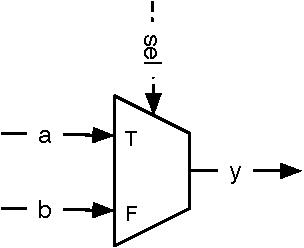
\includegraphics[scale=\scale]{../figures/mux}
\end{figure}
\begin{itemize}
\item A Multiplexer selects between alternatives
\item So common that Chisel provides a construct for it
\item Selects \code{a} when \code{sel} is \code{true.B} otherwise \code{b}
\end{itemize}
\shortlist{../code/mux.txt}
\end{frame}


\begin{frame}[fragile]{Register}
\begin{itemize}
\item A register is a collection of flip-flops
\item Updated on the rising edge of the clock
\item May be set to a value on reset
\end{itemize}
\begin{figure}
  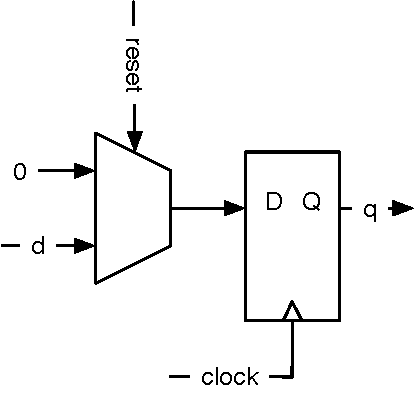
\includegraphics[scale=\scale]{../figures/register-reset-0}
\end{figure}
\end{frame}

\begin{frame}[fragile]{A Register with Reset}
Following code defines an 8-bit register, initialized with 0 at reset:
\shortlist{../code/register.txt}
\noindent An input is connected to the register with the \code{:=} update operator and
the output of the register can be used just with the name in an expression:
\shortlist{../code/reg_con.txt}
\end{frame}

\begin{frame}[fragile]{Reminder: We Construct Hardware}
\begin{itemize}
\item Chisel code looks much like Java code
\item But it is \emph{not} a program in the usual sense
\item It represents a circuit
\item We should be able to \emph{draw} that circuit
\item The ``program'' constructs the circuit
\item All statements are ``executed'' in parallel
\item Statement order has mostly no meaning
\end{itemize}
\end{frame}

\begin{frame}[fragile]{Interlude}
\begin{itemize}
\item Before we look at new material
\item Sprinkle in some info on general development tools
\item Get better at using your computer
\item Learn some tools
\item Don't be afraid of the command line ;-)
\item
\item
\item Engineers are power users!
\end{itemize}
\end{frame}

\begin{frame}[fragile]{What is \code{git}?}
\begin{itemize}
\item \code{git} is a distributed version-control system
\begin{itemize}
\item What does that mean?
\item \href{https://en.wikipedia.org/wiki/Git}{Wikipedia on git}
\item Draw a figure
\end{itemize}
\item To manage source code or other documents
\item Track changes in computer files
\item Created by Linus Torvalds for Linux kernel development
\item Good tool for cooperation
\item Mostly used at the command line
\item But graphical clients are available (i.e., with a GUI)
\end{itemize}
\end{frame}

\begin{frame}[fragile]{What is GitHub?}
\begin{itemize}
\item \href{https://github.com/}{GitHub} is a git repository server
\item GitHub is a classic startup, based in San Francisco
\item Acquired 2018 by Microsoft for \$7.5 billion
\item Many open-source projects are on GitHub (e.g., Chisel)
\begin{itemize}
\item 85 million repositories, and 28 million developers
\end{itemize}
\item Our DE2 material is hosted on GitHub
\begin{itemize}
\item Lab material (you have used it)
\item The slides
\item The Chisel book
\item see \url{https://github.com/schoeberl}
\item Everyone can contribute via GitHub ;-)
\end{itemize}
\end{itemize}
\end{frame}


\begin{frame}[fragile]{Comment on Character Usage and Language}
\begin{itemize}
\item Computers used for long time ASCII characters
\item Show \href{http://www.asciitable.com/}{ASCII table}
\item Does NOT contain the special letters of DK, SE, AT,...
\item Only a subset of ASCII was allowed for identifiers
\item Languages such as Java or Scala are now more tolerant
\begin{itemize}
\item You could use Chinese characters for your Java program!
\end{itemize}
\item Please do not use any special characters
\begin{itemize}
\item Also not in file names
\end{itemize}
\item Programming is international
\begin{itemize}
\item Use English identifiers and comments
\end{itemize}
\item Avoid spaces in file names and folders
\end{itemize}
\end{frame}

\begin{frame}[fragile]{Coding Style}
\begin{itemize}
\item Similar to Java
\item Use readable, meaningful names
\begin{itemize}
\item E.g., \code{sum} instead of \code{y}
\end{itemize}
\item Use \code{camelCase} for identifiers
\item \code{Modules} (classes) start with uppercase
\begin{itemize}
\item E.g., \code{VendingMachine}
\end{itemize}
\item Mark you register with a postfix \code{Reg}
\begin{itemize}
\item E.g., \code{countReg}
\end{itemize}
\item Use consistent indentation
\begin{itemize}
\item Chisel style is 2 spaces (blanks)
\end{itemize}
\item Use ASCII only ;-)
\end{itemize}
\end{frame}

\begin{frame}[fragile]{Combinational Circuits}
\begin{itemize}
\item Simplest is a Boolean expression
\item Assigned a name (\code{e})
\item This expression can be reused in another expression
\end{itemize}
\shortlist{../code/comb_bool.txt}
\end{frame}

\begin{frame}[fragile]{Fixed Expression}
\begin{itemize}
\item Expression is fixed
\item Trying to reassign with \code{=} results in an error
\item Trying the Chisel conditional update \code{:=} results in runtime error
\end{itemize}
\shortlist{../code/comb_bool.txt}
\shortlist{../code/comb_error.txt}
\end{frame}

\begin{frame}[fragile]{Combinational Circuit with Conditional Update}
\begin{itemize}
\item Chisel supports conditional update
\item Value first needs to be wrapped into a \code{Wire}
\item Updates with the Chisel update operation \code{:=}
\item With \code{when} we can express a conditional update
\item The resulting circuit is a multiplexer
\item The rule is that the last enabled assignment counts
\begin{itemize}
\item Here the order of statements has a meaning
\end{itemize}
\end{itemize}
\shortlist{../code/comb_wire.txt}
\end{frame}

\begin{frame}[fragile]{The ``Else'' Branch}
\begin{itemize}
\item We can express a form of ``else''
\item Note the \code{.} in \code{.otherwise}
\end{itemize}
\shortlist{../code/comb_otherwise.txt}
\end{frame}


\begin{frame}[fragile]{A Chain of Conditions}
\begin{itemize}
\item To test for different conditions
\item Select with a priority order
\item The first that is true counts
\item The hardware is a chain of multiplexers
\end{itemize}
\begin{columns}
\column{0.5\textwidth}
\shortlist{../code/comb_elsewhen.txt}
\column{0.5\textwidth}
\begin{figure}
  \includegraphics[scale=\scale]{../figures/mux-chain}
\end{figure}
\end{columns}
\end{frame}

\begin{frame}[fragile]{Default Assignment}
\begin{itemize}
\item Practical for complex expressions
\item Forgetting to assign a value on all conditions
\begin{itemize}
\item Would describe a latch
\item Runtime error in Chisel
\end{itemize}
\item Assign a default value is good practise
\end{itemize}
\shortlist{../code/comb_wiredefault.txt}
\end{frame}

\begin{frame}[fragile]{Logic Can Be Expressed as a Table}
\begin{itemize}
\item Sometimes more convenient 
\item Still combinational logic (gates)
\item Is converted to Boolean expressions
\item Let the synthesize tool do the conversion!
\item We use the \code{switch} statement
\end{itemize}
\shortlist{../code/encdec_dec.txt}
\end{frame}


\begin{frame}[fragile]{A Decoder}
\begin{figure}
  \includegraphics[scale=\scale]{../figures/decoder}
\end{figure}
\begin{itemize}
\item Converts a binary number of $n$ bits to an $m$-bit signal, where $m \leq 2^n$
\item The output is one-hot encoded (exactly one bit is one)
\item Building block for a $m$-way Mux
\item Used for address decoding in a computer system
\end{itemize}
\end{frame}

\begin{frame}[fragile]{Truth Table of a Decoder}
\begin{table}
  \begin{tabular}{rr}
    \toprule
    a & b \\
    \midrule
    00 & 0001 \\
    01 & 0010 \\
    10 & 0100 \\
    11 & 1000 \\
    \bottomrule 
  \end{tabular} 
\end{table}
\begin{itemize}
\item Does this look like the table we have seen?
\end{itemize}
\end{frame}

\begin{frame}[fragile]{Decoder in Chisel}
\begin{itemize}
\item Binary strings are a clearer representation
\end{itemize}
\shortlist{../code/encdec_decbin.txt}
\end{frame}

\begin{frame}[fragile]{An Encoder}
\begin{figure}
  \includegraphics[scale=\scale]{../figures/encoder}
\end{figure}
\begin{itemize}
\item Converts one-hot encoded signal
\item To binary representation
\end{itemize}
\end{frame}

\begin{frame}[fragile]{Truth Table of an Encoder}
\begin{table}
  \begin{tabular}{rr}
    \toprule
    a & b \\
    \midrule
    0001 & 00 \\
    0010 & 01 \\
    0100 & 10 \\
    1000 & 11 \\
    ???? & ?? \\
    \bottomrule 
  \end{tabular} 
\end{table}
\begin{itemize}
\item Only defined for one-hot input
\end{itemize}
\end{frame}

\begin{frame}[fragile]{Encoder in Chisel}
\begin{itemize}
\item We cannot describe a function with undefined outputs
\item We use a default assignment of \code{"b00"}
\end{itemize}
\shortlist{../code/encdec_enc.txt}

\end{frame}

\begin{frame}[fragile]{Register (Again)}
\begin{itemize}
\item Sequential building blocks
\begin{itemize}
\item Contain a register
\item Plus combinational circuits
\end{itemize}
\end{itemize}
\begin{figure}
  \includegraphics[scale=\scale]{../figures/register}
\end{figure}
\shortlist{../code/sequ_reg.txt}
\end{frame}



\begin{frame}[fragile]{Register in Two Steps}
\shortlist{../code/sequ_reg2.txt}
\end{frame}

\begin{frame}[fragile]{Register With Reset}
\begin{figure}
  \includegraphics[scale=\scale]{../figures/register-reset}
\end{figure}
\shortlist{../code/sequ_reg_init.txt}
\end{frame}

\begin{frame}[fragile]{Timing Diagram of the Register with Reset}
\begin{figure}
  \includegraphics[scale=1]{../figures/reg_wave}
\end{figure}
\begin{itemize}
\item Also called waveform diagram
\item Logic function over time
\item Can be used to describe a circuit function
\item Useful for debugging
\end{itemize}
\end{frame}

\begin{frame}[fragile]{Register with Enable}
\begin{figure}
  \includegraphics[scale=\scale]{../figures/register-enable}
\end{figure}
\begin{itemize}
\item Only when \code{enable} true is a value is stored
\end{itemize}
\shortlist{../code/sequ_reg_ena.txt}

\end{frame}

\begin{frame}[fragile]{Timing Diagram for an Enable Register}
\begin{figure}
  \includegraphics[scale=1]{../figures/reg_en_wave}
\end{figure}
\end{frame}

\begin{frame}[fragile]{More on Register}
\begin{itemize}
\item We can combine initialization and enable
\end{itemize}
\shortlist{../code/sequ_reg_init_ena.txt}
\begin{itemize}
\item A register can also be part of an expression
\item What does the following circuit do?
\end{itemize}
\shortlist{../code/sequ_reg_rising.txt}
\end{frame}


\begin{frame}[fragile]{Combine a Register with an Adder}
\begin{figure}
  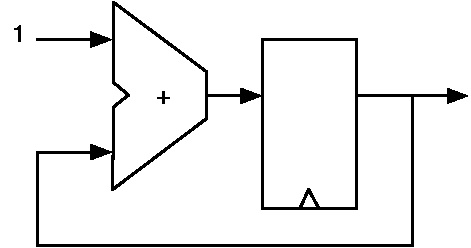
\includegraphics[scale=\scale]{../figures/counter}
\end{figure}
\begin{itemize}
\item Is a free running counter
\item 0, 1, ... 14, 15, 0, 1, ...
\end{itemize}
\shortlist{../code/sequ_free_counter.txt}
\end{frame}


\begin{frame}[fragile]{A Counter}
\shortlist{../code/counter.txt}
\begin{itemize}
\item This counter counts from 0 to 9
\item And starts from 0 again after reaching 9
\begin{itemize}
\item Starting from 0 is common in computer engineering
\end{itemize}
\item A counter is the hardware version of a \emph{for loop}
\item Often needed
\item Can you draw the schematic?
\end{itemize}
\end{frame}

\begin{frame}[fragile]{Counting Events}
\begin{figure}
  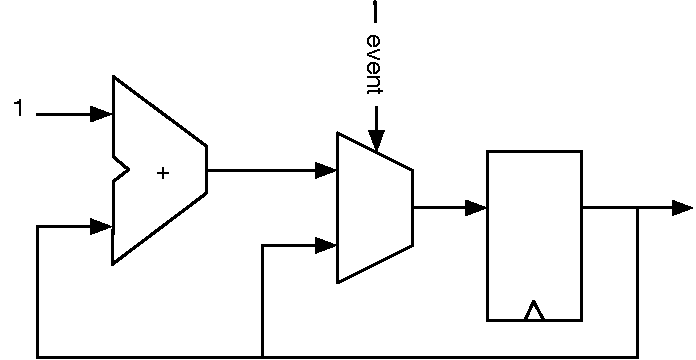
\includegraphics[scale=\scale]{../figures/event-counter}
\end{figure}
\begin{itemize}
\item Is the schematics and the code the same?
\end{itemize}
\shortlist{../code/sequ_event_counter.txt}
\end{frame}


\begin{frame}[fragile]{Structure With Bundles}
\begin{itemize}
\item A \code{Bundle} to groups signals
\item Can be different types
\item Defined by a class that extends \code{Bundle}
\item List the fields as \code{val}s within the block
\end{itemize}
\shortlist{../code/bundle.txt}
\end{frame}

\begin{frame}[fragile]{Using a Bundle}
\begin{itemize}
\item Create it with \code{new}
\item Wrap it into a \code{Wire}
\item Field access with \emph{dot} notation
\end{itemize}
\shortlist{../code/bundle_use.txt}
\end{frame}

\begin{frame}[fragile]{A Collection of Signals with \code{Vec}}
\begin{itemize}
\item Chisel \code{Vec} is a collection of signals of the same type
\item The collection can be accessed by an index
\item Similar to an array in other languages
\end{itemize}
\shortlist{../code/vec.txt}
\end{frame}

\begin{frame}[fragile]{Using a \code{Vec}}
\shortlist{../code/vec_access.txt}
\begin{itemize}
\item Reading from an \code{Vec} is a multplexer
\item We can put a \code{Vec} into a \code{Reg}
\end{itemize}
\shortlist{../code/reg_file.txt}
\noindent An element of that register file is accessed with an index and used as a normal register.

\shortlist{../code/reg_file_access.txt}
\end{frame}


\begin{frame}[fragile]{Mixing Vecs and Bundles}
\begin{itemize}
\item We can freely mix bundles and vectors
\item When creating a vector with a bundle
type, we need to pass a prototype for the vector fields. Using our
\code{Channel}, which we defined above, we can create a vector of channels with:
\end{itemize}
\shortlist{../code/vec_bundle.txt}
\begin{itemize}
\item A bundle may as well contain a vector
\end{itemize}
\shortlist{../code/bundle_vec.txt}
\end{frame}

\begin{frame}[fragile]{Lab Today}
\begin{itemize}
\item Combinational circuits in Chisel
\item \href{https://github.com/schoeberl/chisel-lab/tree/master/lab2}{Lab 2 Page}
\item You need to download again, as I have updated the lab
\begin{itemize}
\item Or learn to use git and do a  \code{git pull} ;-)
\end{itemize}
\item Each exercise contains a test, which initially fails
\item \code{sbt test} runs them all
\begin{itemize}
\item To just run a single test, run e.g.,\\
\code{sbt "testOnly MajorityPrinter"}
\end{itemize}
When all test succeed your are done ;-)
\item Components contain a comment where you shall add your implementation
\item The initial majority example has an optional implementation in an FPGA
\end{itemize}
\end{frame}

\begin{frame}[fragile]{Summary}
\begin{itemize}
\item Think in hardware
\begin{itemize}
\item Draw ``boxes''
\end{itemize}
\item Combinational logic (= Boolean function)
\begin{itemize}
\item Logical and arithmetic expressions
\item Conditional update (\code{when})
\item Function tables with \code{switch}
\item Large multiplexer with a \code{Vec}
\end{itemize}
\item Registers
\begin{itemize}
\item Define as \code{Reg}, \code{RegNext}, or \code{RegInit}
\end{itemize}
\end{itemize}
\end{frame}

\begin{frame}[fragile]{Summary}
\begin{itemize}
\item We looked at basic digital circuit blocks
\item Now you know all you need to build any digital circuit!
\begin{itemize}
\item Digital controller
\item MP3 player
\item Microprocessor
\item Data center accelerator
\item ...
\end{itemize}
\item Will show you some constructs for a more \emph{elegant} style
\item Next lecture is given by Jens Sparsoe and is on timing
\end{itemize}
\end{frame}


\end{document}

\begin{frame}[fragile]{Summary}
\begin{itemize}
\item abc
\end{itemize}
\end{frame}
